% Options for packages loaded elsewhere
\PassOptionsToPackage{unicode}{hyperref}
\PassOptionsToPackage{hyphens}{url}
%
\documentclass[
]{article}
\usepackage{amsmath,amssymb}
\usepackage{lmodern}
\usepackage{iftex}
\ifPDFTeX
  \usepackage[T1]{fontenc}
  \usepackage[utf8]{inputenc}
  \usepackage{textcomp} % provide euro and other symbols
\else % if luatex or xetex
  \usepackage{unicode-math}
  \defaultfontfeatures{Scale=MatchLowercase}
  \defaultfontfeatures[\rmfamily]{Ligatures=TeX,Scale=1}
\fi
% Use upquote if available, for straight quotes in verbatim environments
\IfFileExists{upquote.sty}{\usepackage{upquote}}{}
\IfFileExists{microtype.sty}{% use microtype if available
  \usepackage[]{microtype}
  \UseMicrotypeSet[protrusion]{basicmath} % disable protrusion for tt fonts
}{}
\makeatletter
\@ifundefined{KOMAClassName}{% if non-KOMA class
  \IfFileExists{parskip.sty}{%
    \usepackage{parskip}
  }{% else
    \setlength{\parindent}{0pt}
    \setlength{\parskip}{6pt plus 2pt minus 1pt}}
}{% if KOMA class
  \KOMAoptions{parskip=half}}
\makeatother
\usepackage{xcolor}
\IfFileExists{xurl.sty}{\usepackage{xurl}}{} % add URL line breaks if available
\IfFileExists{bookmark.sty}{\usepackage{bookmark}}{\usepackage{hyperref}}
\hypersetup{
  pdftitle={How has the Brazilian Amazon been constructed as a problem? An analysis of presidential speeches since 1985},
  pdfauthor={Livio Silva-Muller; Henrique Sposito},
  hidelinks,
  pdfcreator={LaTeX via pandoc}}
\urlstyle{same} % disable monospaced font for URLs
\usepackage[margin=1in]{geometry}
\usepackage{longtable,booktabs,array}
\usepackage{calc} % for calculating minipage widths
% Correct order of tables after \paragraph or \subparagraph
\usepackage{etoolbox}
\makeatletter
\patchcmd\longtable{\par}{\if@noskipsec\mbox{}\fi\par}{}{}
\makeatother
% Allow footnotes in longtable head/foot
\IfFileExists{footnotehyper.sty}{\usepackage{footnotehyper}}{\usepackage{footnote}}
\makesavenoteenv{longtable}
\usepackage{graphicx}
\makeatletter
\def\maxwidth{\ifdim\Gin@nat@width>\linewidth\linewidth\else\Gin@nat@width\fi}
\def\maxheight{\ifdim\Gin@nat@height>\textheight\textheight\else\Gin@nat@height\fi}
\makeatother
% Scale images if necessary, so that they will not overflow the page
% margins by default, and it is still possible to overwrite the defaults
% using explicit options in \includegraphics[width, height, ...]{}
\setkeys{Gin}{width=\maxwidth,height=\maxheight,keepaspectratio}
% Set default figure placement to htbp
\makeatletter
\def\fps@figure{htbp}
\makeatother
\setlength{\emergencystretch}{3em} % prevent overfull lines
\providecommand{\tightlist}{%
  \setlength{\itemsep}{0pt}\setlength{\parskip}{0pt}}
\setcounter{secnumdepth}{-\maxdimen} % remove section numbering
\newlength{\cslhangindent}
\setlength{\cslhangindent}{1.5em}
\newlength{\csllabelwidth}
\setlength{\csllabelwidth}{3em}
\newlength{\cslentryspacingunit} % times entry-spacing
\setlength{\cslentryspacingunit}{\parskip}
\newenvironment{CSLReferences}[2] % #1 hanging-ident, #2 entry spacing
 {% don't indent paragraphs
  \setlength{\parindent}{0pt}
  % turn on hanging indent if param 1 is 1
  \ifodd #1
  \let\oldpar\par
  \def\par{\hangindent=\cslhangindent\oldpar}
  \fi
  % set entry spacing
  \setlength{\parskip}{#2\cslentryspacingunit}
 }%
 {}
\usepackage{calc}
\newcommand{\CSLBlock}[1]{#1\hfill\break}
\newcommand{\CSLLeftMargin}[1]{\parbox[t]{\csllabelwidth}{#1}}
\newcommand{\CSLRightInline}[1]{\parbox[t]{\linewidth - \csllabelwidth}{#1}\break}
\newcommand{\CSLIndent}[1]{\hspace{\cslhangindent}#1}
\usepackage{booktabs}
\usepackage{longtable}
\usepackage{array}
\usepackage{multirow}
\usepackage{wrapfig}
\usepackage{float}
\usepackage{colortbl}
\usepackage{pdflscape}
\usepackage{tabu}
\usepackage{threeparttable}
\usepackage{threeparttablex}
\usepackage[normalem]{ulem}
\usepackage{makecell}
\usepackage{xcolor}
\ifLuaTeX
  \usepackage{selnolig}  % disable illegal ligatures
\fi

\title{How has the Brazilian Amazon been constructed as a problem? An
analysis of presidential speeches since 1985}
\author{Livio Silva-Muller\footnote{Phd Candidate, The Geneva Graduate
  Institute ,
  \href{mailto:livio.silva@graduateinstitute.ch}{\nolinkurl{livio.silva@graduateinstitute.ch}}} \and Henrique
Sposito\footnote{Phd Candidate, The Geneva Graduate Institute Geneva,
  \href{mailto:henrique.sposito@graduateinstitute.ch}{\nolinkurl{henrique.sposito@graduateinstitute.ch}}}}
\date{April 2022}

\begin{document}
\maketitle
\begin{abstract}
This paper \ldots{}
\end{abstract}

\pagebreak

\hypertarget{introduction}{%
\section{1 Introduction}\label{introduction}}

The Amazon needs to be protected from foreign interests. The Amazon
needs to be exploited for its natural resources. The Amazon needs to be
preserved as a standing ecosystem. Historically, different Brazilian
federal government proposed diverse policies to deal with the Amazon.
Each of these policies contain an implicit assumption of what needs to
be solved, or in other words, it represents the region, the forest, or
its peoples as a particular problem. In the three examples above, the
Amazon is represented as an issue of national sovereignty, economic
integration, and environmental conservation, respectively. Each of these
constructions, and their proposed solutions, have been described as
policy cycles of Brazilian governments (Acker 2014; Hecht and Cockburn
1990; Hochstetler and Keck 2007). However, policy cycles are usually
represented monolithically, advancing a view that specific governments
see the Amazon as an instance of only one specific problem. Albeit the
current calls to understand the environment as a social-cultural
construction and to identify the effect of culture on environmental
outcomes (Waroux et al. 2021), we lack empirical accounts of how the
Brazilian Amazon has been constructed as a problem over time, by
geographical location, and between and within governments

In this article, we investigate how the Brazilian Amazon has been
constructed as a problem in political discourses. Building on Hirschman
(1963) concept of chosen problems in policy making, we propose a
framework to identify how problem-construction. Although
problem-construction takes place in a series of instances (e.g.~policy
committees, legislative bodies, media, etc.), we analyze the case of
political discourse by Brazilian presidents since 1985. We opt for
presidential speeches for three reasons. First, political discourses at
the top have the power to introduce and justify public policy, as well
as shape its perception to broad audiences (Zarefsky 2004). In turn,
policy perception is key for policy adoption and implementation (Alesina
and Giuliano 2009; López et al. 2020). The literature has shown that
deforestation rates in Brazil are more responsive to the government's
environmental policy than exogenous factors as market fluctuations
(Assunção, Gandour, and Rocha 2015; Capobianco 2019, 2021). Thus,
understanding how policy comes about discursively is important. Second,
environmental discourse at the top can help expand or restrict what
types of behaviors are accepted in the ground. When Brazilian presidents
speak about the Amazon it not only makes headlines, nationally and
internationally(Brice and Smith 2021; Harris 2021; Miranda 2021), but
also incites responses, shapes expectations, and feeds into the behavior
of many actors involved in the Amazon, from investors to agribusiness to
local farmer. This is especially pertinent for deforestation as previous
research found that policy expectations, generated from material and
discursive governmental practices, are a crucial factor in decisions to
deforest at the ground (Capobianco 2019; Campbell 2015). Unpacking
discourse at the top might help us raise hypotheses about environmental
outcomes that are culturally situated. Finally, as our theoretical
framework suggests, problem-construction varies by geographic location.
Presidential discourses take place in a series of sites with diverse
audiences: from launching a new bridge in a small municipality in the
middle of the Amazon, to a keynote speech in a business association in
São Paulo, to the UN general assembly in New York. Working with
presidential discourses allows us to identify this variation in
meaningful ways and better how the Amazon is socially constructed.

To investigate how the Brazilian Amazon has been constructed as a
problem in political discourses, we create a dataset containing 6130
official presidential speeches by all Brazilian presidents since 1985.
We subset the dataset by identifying Amazonian related statements within
these speeches. We find that 2014 sections in these discourses refer to
the Amazon at least once. We then develop a codebook grounded on
Amazonian historiography to code how each of these statements constructs
the Amazon as a particular problem. We use this codebook to manually
code a randomly selected training set of the Amazonian related
statements. Using R, we then train a supervised machine-learning model
in the hand-coded set and automatically label the remaining set of
Amazonian statements. We then conduct a descriptive and inferential
analysis of this data, tying our findings to endogenous and exogenous
events related to deforestation.

Our findings are threefold. First, endogenous events as the death of
Chico Mendes, the 1992 Earth Summit, the 2009 Copenhaguen Summit, the
2015 Paris Summit, and the 2021 London Summit drive generally the
interest in the Amazon. That seems to be the case even after controlling
share of annual speeches mentioning the Amazon for deforestation,
inflation, and speaker. Second, there was a sharp decrease in economic
related problem-constructions from the late 1990 to 2010, matched by an
increase in speeches that construct the Amazon as a problem of social
development and environmental conservation. This trend is reversed in
the late 2010s, with the twist of sovereignty making a strong comeback.
Finally, using a multinominal model, we find that the farthest away the
speaker is from the Amazon, be it within the country in non-Amazonian
States or outside Brazil, the more likely the speaker is to construct
the Amazon as a problem of environmental conservation than economic
integration or social development.

This article proceeds as follows: first, we review Amazonian literature
to identify the main policy-cycles and their underlying problem
construction. We then propose a theoretical framework to understand
problem-construction and discourse. In the methodology section, we
operationalize our framework and present the codebook. Section four
portrays our main results. Finally, we conclude by discussing our
findings and proposing future research.

\hypertarget{amazonian-policy-cycles-discourse-and-problem-construction}{%
\section{2 Amazonian policy-cycles, discourse, and
problem-construction}\label{amazonian-policy-cycles-discourse-and-problem-construction}}

\hypertarget{literature-review-policy-cycles-in-the-amazonian-literature}{%
\subsection{2.1 Literature Review: policy-cycles in the Amazonian
literature}\label{literature-review-policy-cycles-in-the-amazonian-literature}}

For the purposes of this article, we understand Amazonian literature as
the body of research by social and environmental scientists that tells
the story of diverse policies adopted to solve problems in the region.
The three main policy-cycles we identify in Amazonian literature are:
national sovereignty, economic integration, and environmental
conservation. We tie each one of them to a specific problem and
consequently a solution. We close the sub-section reviewing the
relationship between policy, presidential discourse, and environmental
problems.

\hypertarget{national-sovereignty}{%
\subsubsection{2.1.1 National sovereignty}\label{national-sovereignty}}

In The Fate of the Forest: Developers, Destroyers, and Defenders of the
Amazon, Hecht and Cockburn write that all over the world tropical
forests are destroyed, but ``what imbues the case of the Amazon with
such passion is the symbolic content of the dreams it ignites'' (1990,
1). It started with the first natural history of the New World, by
Oviedo in 1535, who recounts the stories of conquest of local
populations and gold hoarders. The dream of fortunes to be found in the
Eldorado composed the imaginaries of \emph{bandeirantes}\footnote{\emph{Bandeirantes}
  means ``flag-carriers'', the word is used to designate Portuguese
  colonials and later Brazilian explorers, expanding the Brazilian
  territory beyond what the Tordesillas Treaty established. The treaty
  allocated almost the whole Amazonian territory to the Spanish Empire,
  the bandeirantes took much of the territory afterwards.} from the
southeast of Brazil and colonizers from everywhere else. It rendered the
territory the venue for aspiration and object of an intense scramble in
the subsequent centuries, defined as ``a (\ldots) form of nation
building (\ldots)'' (Hecht and Cockburn 1990, preface). The Portuguese
empire and subsequently the Brazilian monarchy were concerned with
establishing their territory. In the process of securing Amazonian
borders, Brazil thwarted ``the imperial ambitions of France, Britain,
the United States, Belgium, Bolivia, and Peru'' (Hecht 2013, 8), and
when the dust settled and the scramble was over, half of the Amazon
emerged Brazilian. While Brazilian military diplomacy was very
successful, the process did not come without its traumas. A significant
experience were the negotiations with Bolivia in 1902 to secure the
Amazonian state of Acre, during which they found out about American
attempts to trick Brazil(Hecht and Cockburn 1990). This case was still
part of the memory of the generals who led the country during the
military dictatorship of 1964 and wanted to protect Brazil's sovereignty
over the Amazon from the communist threat during the Cold War(Garfield
2013).

As we move from a world where non-state actors gain importance in
environmental governance and international politics generally
(Silva-Muller and Faul 2022; Andonova 2014; Westerwinter 2021), the
sovereignty problem becomes more varied. Multiple non-state actors
(NGOs, foundations, IOs, and so on) join the conversation about
Amazonian policies more substantially as the military dictatorship
starts to end (Hochstetler 2021; Capobianco 2019; Franchini and Viola
2019). Threads to national sovereignty, consequently, can be interpreted
as coming from a different set of actors than before. Allegedly false
claims about the Brazilian Amazon in international and domestic fora,
for instance, are often tied to strategies of `internationalizing' the
Amazon. This might come both from foreign actors as well as domestic
non-state actors. Relatedly, mentions of Amazonian myths which have been
debunked as the `Earth of the Lungs', are also tied to
internationalizing strategies.

The sovereignty problem advances the view that the Brazilian Amazon is
Brazilian and foreign presence, non-state presence and alleged lies are
part of a broader strategy to internationalize the region. The policy
solutions relate to close monitoring of the borders, strict regimes
related to entry in the region, and combating alleged disinformation
about the Amazon nationally and internationally.

\hypertarget{economic-integration}{%
\subsubsection{2.1.2 Economic integration}\label{economic-integration}}

The Vargas dictatorship (1937-46) and the military dictatorship
(1964-89) took over the task of modernizing the Amazon. In 1966, the
Brazilian Military launched Operation Amazon, a policy to modernize the
region based on a set of assumptions (Acker 2014). First, nature should
be conquered by men. Second, exploiting natural resources would render
the Amazon region a global powerhouse. Third, such a project would
integrate the region with the rest of the country. Concretely, this
meant a series of infrastructure projects, such as roads and dams,
incentives for settlers to develop ranches and expand the agricultural
frontier, as well as establishing tax free zones to attract industry.
The capital to conduct such changes, paradoxically, came from national
and international sources (Acker 2014), leading to a series of national
and international enterprises settling in the Amazon region. Capobianco
(2019) describes the period from the 1950-80 in a similar fashion,
referring to a wider range of policies of economic integration: the 1953
Plano de Valorização Econômica da Amazônia; the 1966 Superintendência do
Desenvolvimento da Amazônia; the 1967 Superintendência da Zona Franca de
Manaus; the 1970 Plano de Integração Nacional; the 1975 Programa
Polamazônia; the 1980s Programa Grande Carajás and Programa Calha Norte;
among others.

The economic integration problem advances the view that the Brazilian
Amazon needs to be developed and modernized. The policy solution relates
to the creation of a series of policies, often centralized by the
federal government and thus external to the region (Becker 2005), that
have at its core the development of the necessary infrastructure
(physical, fiscal, or monetary) to integrate the region in the national
and international economy.

\hypertarget{environmental-conservation}{%
\subsubsection{2.1.3 Environmental
conservation}\label{environmental-conservation}}

The rapid economic changes in the region in the 1960s, 1970s, and 1980s
were matched with the birth of environmental institutions such as the
New Forest Code (1964), the Secretary of Environment (1973), and the
National Environment Law (1980) (Drummond and Barros-Platiau 2006). A
common explanation for these institutions in the Amazonian literature is
the impression of lack of control after years of centalized economic
integration policies (Acker 2021; Capobianco 2021; Hecht and Cockburn
1990). As deforestation, fires, and violence rose in the region,
catching international attention, the military government deemed as
necessary the establishment of an environmental bureaucracy. This
process accelerated in the late 1980s, with the birth of modern
environmentalism epitomized in the 1992 Earth Summit in Rio de Janeiro
(Hochstetler 2021; Capobianco 2021). Hochstetler and Keck (2007) argue
that during preparations for the summit, a new form of Brazilian
environmentalism emerged: socio-environmentalism. They define it as an
emphasis on local livelihoods of people while protecting nature.
Capobianco (2019) argues in a similar line, establishing
socio-environmentalism as the main government response in the 1990s and
early 2000s in a series of policies: the 2001 Sistema Nacional de
Unidades de Conservação; the 2003 Programa Amanônia Sustentavel; the
2004 Plano de Ação para a Prevenção e Controle do Desmatamento na
Amazônia Legal; the 2004 Plano BR-163 Sustentável; the 2010 Lei Nacional
das Mudanças Climáticas; among others.

The conservationist problem-construction advances the view that Amazon
should be preserved, deforestation should be halted, and the sustainable
practices of indigenous and local peoples should be maintained through
protection of their territories and rights to self-determination
(Hochstetler and Keck 2007). The policy solution implies more investment
in command-and-control infrastructure (as remote-sensing technology for
environmental outcome measurement), more investment in the valuation of
standing ecosystems through incentive schemes, and more policies
facilitating indigenous environmental practices.

\hypertarget{policy-and-discourse}{%
\subsubsection{2.1.4 Policy and discourse}\label{policy-and-discourse}}

Different authors have proposed similar periodization for policy-cycles
in the Amazon: a focus on sovereignty until the military dictatorship of
1964, followed by strong economic integration policies until the mid
1980s, and finally a shift to conservation after the 1992 Earth Summit.
At the macro-historical level, the wider Amazonian vision of the 1964
military dictatorship, encompassed by the whole group of policies they
adopted, for instance, did favor economic integration. Nevertheless, at
the level of policies adopted, there is more variation than these
periods would suggest. For example, the 1980 Programa Calha Norte did
contain elements to ensure sovereignty, integrate the region to the
country's economy, and preserve the forest. Framing this policy as an
issue of economic integration, then, can be seen as a choice.

Hence, while the literature might represent governments as coherent
proponents of a particular policy retroactively, political actors might
have adopted strategies that outline problem-constructions of policies
differently. For historical inquiry, it is important to periodize policy
cycles comprehensively. We largely agree with what the literature
assigns to previous governments. However, the possibility of varied
portrayals of the same policy opens up an understanding agenda-setting
and policy-adoption that is less linear.

Problem-construction at the level of discourse is also more varied. They
are not monolithic in time, across location, or even by the same
speaker. While governmental discourses in Brazil have been studied for
topic such as inflation or race relations \footnote{For an overview on
  how inflation and political discourse in Brazil see Porto (2007),
  Malheiros-Poulet (2012), and Fonseca et al.~(2021). For a few studies
  on racist and anti-racist discourses in Brazil see Htun (2004), Silva
  and Larkins (2019) and Dijk (2020).}, we only find one systematic
analysis of Amazonian discourse. Barros (2020) investigates Amazonian
discourse in the Brazilian Congress with the objective of identifying
the arguments put forth by congressmen. The main finding is that the
economic value of the Amazon for the cattle industry is the most salient
narrative, leading the author to conclude there is a mismatch between
the international debate (which focuses on preservation) and the
national debate (which focuses on economic development).

We also find several analyzes of environmental discourse in American
presidential speeches. Calderwood (2019) examines 2919 mentions of
climate change in American official presidential speeches since 1989.
Among various findings, one that stands out is that American presidents
frequently side-step the environmental aspects of climate change (ibid).
He also identifies a shift from economic to security framing of climate
issues, side-lining its environmental aspects. In another article,
Calderwood (2020) tests the effect of geographic location and type of
communication regarding climate change. Building prominently on Putnam
(1988) but also others, he hypothesizes that presidents are more likely
to mention climate change in foreign locations, and that location
influences the specific discursive approach and tone they adopt. He
finds evidence in support of his hypothesis, suggesting American
presidential discourse at the top on climate change does change based on
location. Another example is Bevitori (2015), who investigates how the
`environment' has been constructed in American presidential discourse
since 1960 using a more automated approach. The author finds that
mentions of the environment are typically co-selected with the pronoun
`our', as well as with `economy', `clean', and `preserve'.

While these findings hold for the US, they suffice to argue that
presidents can raise different points about the Amazon at local,
national, or international settings, depending on who they assume their
audience is at that specific instance. That entails the same president
can combine, substitute, or change how they talk about the Amazon and
these views can reflect, or not, the current political scenario, issues
in the agenda, or talk to a different policy cycle at times.

\hypertarget{theoretical-framework-problem-construction-and-presidential-discourse}{%
\subsection{2.2 Theoretical framework: problem-construction and
presidential
discourse}\label{theoretical-framework-problem-construction-and-presidential-discourse}}

In ``Journey towards Progress'', Hirschman (1963) analyzes three policy
problems in three different Latin American countries. The author draws a
conceptual distinction between pressing problems (pressured from outside
parties to the government) and chosen problems (chosen by the government
at their own discretion). Pressing problems can be either privileged or
neglected depending on the degree of pressure exercised by the
interested group. Problems can change from pressing to chosen across
time and in space as a function of solutions becoming available,
changing level of government control in society, or top policymakers
shifting interests (Hirschman 1963, 388--91). Choosing a problem,
though, entails a decision on how to represent it (Bacchi 2009). As
Bacchi puts ``policy has a cultural dimension. It takes shape within
specific historical and national or international contexts'' (2009, 10).
The existence or proposal of a policy generally implies that there is a
(public) problem that needs (governmental) action to be fixed. The
alleged problem is not always explicitly stated in policy. Hirschman
exemplifies chosen problems with the case of the construction of
Brasilia (1975, 388). But building Brasilia can solve a problem of
regional inequality, a problem of a dormant economy without state
investment, a problem of political representation, or all three. How to
represent a policy is a matter of choice. And different representations
speak to different audiences.

We understand that depending on how the problem is represented to be, it
can be a solution of problems that are considered pressing. Different
problem-constructions can address the demands of different
constituencies and it is up to the discretion of the political actor to
construct a particular problem in a particular way given context.
Problem-construction takes place in different sites: national media,
legislative bodies, international fora, policy committees, among others.
What eventually becomes policy is a product of a multi-faceted process
in all these different sites. One avenue through which governments can
emphasize the representations of a problem is discourse. We assume that
problem-construction at the level of discourse is varied. They are not
monolithic in time, across location, or even by the same speaker.

We argue that presidents can employ specific problem-constructions that
build objects as specific problems depending on the context. In the
specific case of the Brazilian Amazon, we contend that Amazonian
problem-construction connect the region to issues of sovereignty,
economic integration, social development, or environmental conservation.
Presidents choose to represent the region as a particular problem. As
Bacchi (2009), we argue that problem-constructions touch on shared
meanings about the region that are available to the speaker as part of
larger social-cultural history. Thus, the ways a president speaks are
culturally and historically mediated and need to be embedded in the
wider history of the region and country. We consider this an advancement
in relation to scholars looking at American presidential speeches, as
they just count mentions to climate change (Calderwood 2019, 2020; Brown
and Sovacool 2017) or environment (Bevitori 2015) without embedding them
in the histories of the issue in the country.

These are the cornerstones of our framework: while governments are
sometimes portrayed as proponents of a specific policy-solution, the way
they construct the Amazon as a problem varies. The specific
problem-constructions that we propose are embedded in Amazonian
historiography and connect presidential speeches to Brazilian larger
social-cultural history. We propose a framework to understand variation
in problem-construction as a choice that is responsive to geographic
location, time, and speaker.

\hypertarget{research-design}{%
\section{3 Research Design}\label{research-design}}

To operationalize our theoretical framework, we adopt a mixed-methods
approach using manual coding and supervised machine learning. We explain
our research design and each step of the procedure in this section.

\hypertarget{data-and-modeling-operationalizing-amazonian-problem-construction}{%
\subsection{3.1 Data and modeling: operationalizing Amazonian problem
construction}\label{data-and-modeling-operationalizing-amazonian-problem-construction}}

We build upon the dataset provided by (Cezar 2020) which contains all
official speeches by Brazilian Presidents from 1985 to 2019 scrapped
from the archives of the Brazilian Presidential Library. We update the
dataset by scraping and adding all official speeches from 2020 and 2021.
The final dataset encompasses 6130 speeches for all the presidents of
Brazil since 1985. We then identify all speeches about the Amazon as a
region, peoples, or forest out of the 6130 speeches. We do so by
detecting all speeches in which the stem ``amazon'' appears. In
Portuguese, the stem captures terms such as ``Amazonia'', ``Amazonica'',
``Amazonidas'', ``Amazonense(s)'', ``Amazonas'', among others. We find
that 946 speeches are, at least partially, about the Amazon from the
6130.

Using the poldis R package, we proceed to extract two sentences before
and two sentences after the sentence in which the stem ``amazon''
appears. We opt for picking two sentences before and two sentences
after, rather than words, because sentences usually contain a cohesive
idea. By doing so we create our unit of analysis: an Amazonian
statement. We use Amazon statements as our unit of analysis for two main
reasons. First, working at the level of statements allows us to identify
only passages that are meaningful for our specific purpose. Second, it
increases the number of our observations and its variety meaningfully,
allowing for more specificity in our analysis. This process yields 2014
unique Amazonian statements across the 946 speeches about the Amazon
identified. When an Amazonian statement contains two or more matches of
the stem ``amazon'', we get two sentences before the first match and two
sentences after the last match. On average, an Amazonian statement
contains 123 words.

After revising the literature (section 2), we selected a random sample
of these Amazonian statements to develop a codebook for identifying how
the Amazon is constructed as a problem in presidential discourse (see
Table 1 below). We understand Amazonian problem-constructions as
Weberian ideal types, that is, an unified analytical construct
portraying a `pure' version of a phenomenon. This serves the purpose of
allocating empirical observations within a range of possibilities. We
identify the three problem-constructions derived from the literature
(national sovereignty, economic integration, and environmental
conservation) in the sample of Amazonian statements. However, in
addition to them, we inductively identified a fourth problem
construction that the literature does not explicitly cover: social
development. Presidents sometimes opt to emphasize the lack of
hospitals, sanitation, and schools in relation to peoples'
constitutional rights when speaking about the Amazon. We saw this code
category as substantially different from the other three, hence, we
created the code category `social development'. In their
conceptualization, each code is mutually exclusive in its
conceptualization, meaning that they cover different forms of
constructing the Amazon as a problem, though each Amazonian statement
might be assigned to one or more codes. A statement can, for example,
construct the Amazon as a problem of sovereignty and a problem of
economic integration or a problem of social development and
conservation. Amazonian statements, thus, can be either coded as a
pure-types or mixed-types.

\begin{longtable}[]{@{}lll@{}}
\caption{Table 1 - Amazonian Problem-Construction
Codebook}\tabularnewline
\toprule
Problem\_Construction & Description & Example \\
\midrule
\endfirsthead
\toprule
Problem\_Construction & Description & Example \\
\midrule
\endhead
National Sovereignty & This code constructs the Amazon region and/or
forest as an issue of national sovereignty. We understand claims of
sovereignty as a particular problem-construction that touches on
imaginaries of external threats to territory. Relatedly, we also
understand sovereignty as raising concerns about wrong perspectives and
criticism from foreign and non-state actors about
governments\textless U+2019\textgreater{} actions related to the
Brazilian Amazon. In all, it advances the view that the Amazon is
Brazilian, foreign, and non-state presence in the region needs to be
monitored closely. & Congressman, the fundamental link for Brazil to
really head in the direction to prosperity. I would like first, Hu
Chunhua, to thank you for the words of your ambassador to Brazil
recognizing our sovereignty over the Amazonian region during that recent
episode in the G7 meeting. I would like to thank the Chinese government.
For us, this type of public acknowledgement is priceless in your words
about this region that is so important to the world and to Brazil.
(Bolsonaro 25/10/2019) \\
Economic Integration & This code constructs the Amazon region and/or
forest as an issue of economic integration. It advances the view that
the Amazon needs to be developed and connected to the national economy.
This includes expanding the agricultural frontier through incentives,
creating a diverse set of infrastructure (roads, dams, internet, radio,
energy), fostering differing industries (tourism, mining, cattle,
agriculture and so on) through tax-free zones, as well as facilitating
the exploitation of natural resources for developmental purposes. & If
you allow me, in the Amazon - which for a long time stayed asleep due to
the lack of coordinated actions - have already taken a few structuring
actions. We, in the Amazon, are connecting Manuas, Boa Vista, Caracarai,
until up there, the red line {[}in a map{]} that goes all the way up in
the direction of Venezuela, that is the so-called BR-174 highway. This
highway will allow production in the Tax Free Zone in MAnaus to be
competitive, not within, but outside, that is the vocation of the the
Tax Free Zone to export; and we can even do it through the Caribbean
(Cardoso 02/07/1997) \\
Social Development & This code constructs the Amazon region and/or
forest as an issue of social development. It advances the view that
Amazon is full of citizens who should have their rights guaranteed. This
refers to the construction of schools and universities (right to
education), of hospitals (right to health), and of housing (right to
house). This also includes guarantees of a dignified life with decent
employment, access to water and sanitation, as well as access to
electricity, internet, radio, and light. Finally, this includes
referrals to culture and the right to vote. & The state does not work
for profits, the state needs to guarantee dignity, we find that a
citizen who lives in the riverside of the Amazon river, 600 kilometers
from Manaus, has the right to have the electricity in their house, to
owe a fridge, to owe a television where to watch the soap operas. We
have invested over 14 billion reais in this program, in three and a half
years. Do you know how many electrical lines we have already built? One
million kilometers of lines. (Lula 20/11/2009) \\
Environmental Conservation & This code constructs the Amazon region
and/or forest as an issue of conservation. This problem-construction
focuses on the value of a standing forest and of the preserved ecosystem
in the region. The conservationist narrative advances the view that
Amazon should be preserved, deforestation should be halted, and the
practices of indigenous and traditional populations should be maintained
and fostered. It advances the view that the emission of greenhouse
gasses should be halted, that renewable energy should be supported, and
that protected areas should be created. & I have put in place emergency
measures, I have suspended the exports of wood logs, I have suspended
the fiscal incentives and credits to projects that could damage the
environment in the amazon and I have made a license mandatory to gold
mining that prohibits utilizing mercury in the process. This began the
restructuring of the governmental system of control and preservation of
the environment, I have created the Brazilian Institute for the
Environment and Natural Resources {[}IBAMA{]}, which will be headed by
Dr.~Mesquita (Sarney 20/07/1989) \\
\bottomrule
\end{longtable}

With the codebook in hands, each one of the authors, separately,
hand-coded the same set of 1007 randomly selected Amazonian statements.
This amount refers to 50\% of all the Amazon Statements identified.
Inter-coder agreement for each of the four main categories was 85\%, on
average. For each non-matching coded observation, the co-authors
discussed and sorted their disagreements. Statements that mention the
stem ``amazon'', but are not about the Brazilian Amazon, for example,
might a greeting to the Governor of the Amazonas, were coded as false
positives. The manually coded data is then randomly divided into a
training set, containing 80\% of the hand-coded observations (806
observations), and a validation set, containing the remaining 20\% of
the hand-coded data (201 observations). The training set is used to
train the supervised machine-learning model that automatically
classifies observations while the validation set is used to make sure
the model fit is appropriate.

We chose to employ a support-vector machine (SVM) algorithm to label
texts, that is, a non-probabilistic linear classifier that classifies
documents by assigning points in mapped space to maximize the gap
between binary categories (Meyer et al. 2021; Noble 2006)\footnote{For
  more information on this please see the extended methodology. The
  document includes a detailed discussion of how the SVM algorithm was
  chosen over other algorithms based on evaluation of performance of
  trained models for labeling the validation set. The extended
  methodology also includes a more detailed codebook table with further
  coding guidelines.}. After the SVM model is trained and tuned, and the
model shows to appropriately fit the validation set, we use the model to
automatically code the remaining 1007 Amazonian statements. The model
was also trained to identify false positive observations, which we chose
to delete for analysis since these are not meaningful statements about
the Amazon. The final dataset for analysis contains 1895 coded Amazonian
statements. Finally, we use poldis once more to extract locations for
all speeches in the data. These locations represent the Brazilian state
in which certain speech was given or an international country.

\hypertarget{analysis-and-limitations}{%
\subsection{3.2 Analysis and
limitations}\label{analysis-and-limitations}}

To analyze our data, we first present a series of different plots on
proportions of Amazonian statements and problem-constructions over time
and by presidents. We control proportions for factors that might affect
the incidence of the Amazon in speeches and portray both real and
controlled curves. To test whether different problem constructions
change according to location, we run a multinomial regression model in
which different problem constructions (as categories) are the dependent
variable and location is the independent variable. We also control for
annual deforestation rates, annual inflation rates, and election years
in the model. We interpret the plots and model considering multiple
Amazon related events and policies over the last 30 years, as well as
their correlations with different presidents and locations, while
embedding problem-construction in contemporary happenings.

These procedures come with its limitations. Our codebook is developed
using specific Amazon related vocabulary. For example, a statement will
be coded as economic integration if it is a meaningful support to the
Zona Franca of Manaus or a Dam in the Amazon. However, the economy is
generally a topic that presidents speak about. Hence, high incidence of
economic integration in Amazonian statements can also be related to the
higher importance of this problem-construction in Brazil in time.
Moreover, we classify statements as Amazonian based on a dictionary
composed of a single lexicon stem: ``amazon''. We chose to do so knowing
that a few speeches about the Amazon might not contain the lexicon
``Amazon'', for example, when the president says, ``the forest'' or
``deforestation''. Hence, we might be missing statements about Amazon
that do not refer to it. However, we consider this safer as we cannot be
sure that mentions of the forest or deforestation do not correspond to
other biomes such as the Cerrado or the Mata Atlantica. Nevertheless,
our dataset covers only what is considered an official remark.
Presidents, though, give interviews, appear in debates, talk at campaign
rallies, and more recently start to appear in social media.
Problem-construction within presidential discourse, thus, also happens
in different sites for which we do not account for in this paper.

\hypertarget{how-has-the-amazon-been-constructed-as-a-problem}{%
\section{4 How has the amazon been constructed as a
problem?}\label{how-has-the-amazon-been-constructed-as-a-problem}}

This section presents the three main findings of our analysis. We open
with a broad overview of the evolution of the incidence of Amazon in all
presidential speeches since 1985. In section 4.2, we focus on speeches
that mention the Amazon, introducing the specific problem-constructions
we presented in section 2.1. Finally, we run a multinomial model to show
how problem constructions change as the speaker moves further away from
the Amazon region.

\hypertarget{the-rises-and-falls-of-the-amazon-as-a-topic-in-presidential-speeches}{%
\subsection{4.1 The rises and falls of the Amazon as a topic in
presidential
speeches}\label{the-rises-and-falls-of-the-amazon-as-a-topic-in-presidential-speeches}}

Figure 1 shows the proportion of speeches that mentions the Amazon in
relation to all speeches in each year. The predicted share curve
controls incidence for deforestation\footnote{The reasoning here is that
  knowledge of high or low deforestation rates might drive presidents to
  speak about the Amazon. Nevertheless, matching deforestation with
  speech dates is a complicated endeavor. INPE published consolidated
  deforestation data with almost two years of delay until 2005
  (Capobianco 2021, 60). Preliminary data was published earlier, but
  with lower degrees of confidence in the findings. For the subsequent
  years, the consolidated figures for a given year came out in August of
  the subsequent year. However, it also seems to be the case that the
  executive government have access to the data before everyone else. In
  addition, other sources indicating if deforestation is going up or
  down, as fire data or lower resolution deforestation data (DETER for
  example), or even other sources, circulated within the year the data
  covered. The year of 1988 is particularly indicative of these
  complications: a report dating 1988 was circulating with deforestation
  and fire figures(Fearnside 1990), and a New York Times article about
  the issue with deforestation rates for 1988 was written with comments
  by an INPE scientist (Simons and Times 1988). Hence, we believe the
  most appropriate way of matching is without any lags on deforestation.},
economic situation, and speaker (see appendix for methodological
details). We observe various local maxima: 1989, 1992, 2005, 2009, 2015,
and 2019. These points coincide with exogenous events that helps us
explain the rises and falls of the Amazon in presidential discourse.

First, we observe a steady increase from about 5\% in 1985 to 32\% 1989.
This is the period when the Brazilian Constitution was being written.
Indigenous and traditional populations were instrumental in advocating
for constitutional environmental rights and protection of their
territories (Hecht and Cockburn 1990). These were eventually enshrined
in article 225, which gives all Brazilians a right to a balanced
environment, and in article 231, which grants indigenous and traditional
populations a right over their territory. Two other factors are likely
to explain this increase: in 1988 Chico Mendes was brutally murdered and
the New York Times published an article with pictures of the Amazon
burning (Simons and Times 1988). Both incidents caught unprecedented
international attention. President Sarney responded to these publicly,
and proposed a new set of policies to address, named Nossa Natureza
(Capobianco 2021).

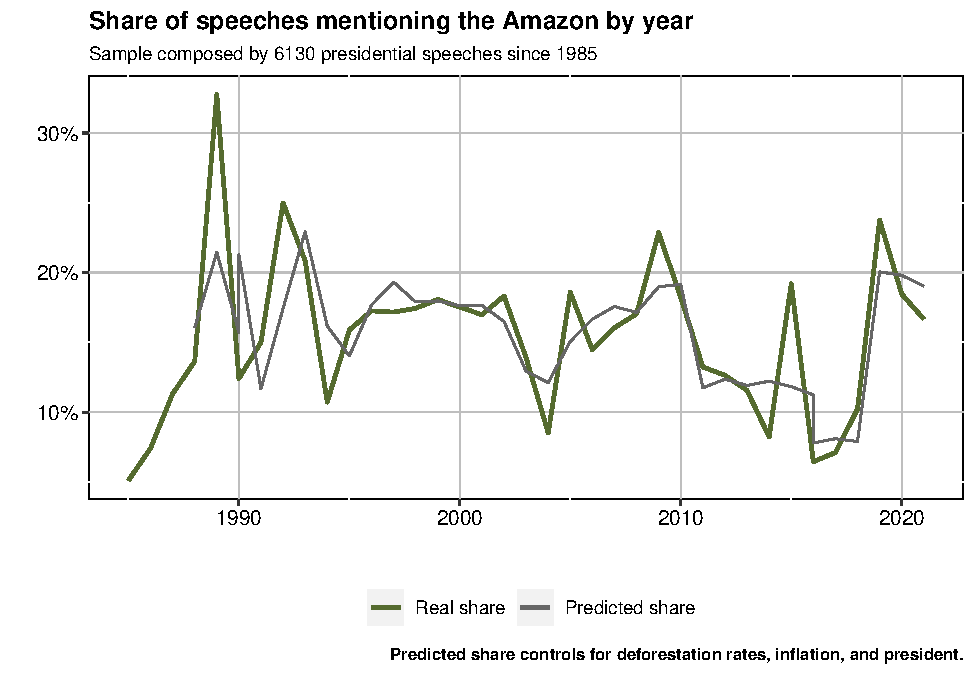
\includegraphics{Full_draft_20220401_files/figure-latex/Figure 1: Amazonian speeches by year-1.pdf}

While in 1990 there was a decrease to about 12.4\%, we observe a novel
increase to 15\% and 25\% in 1991 and 1992 respectively. The driver of
this increase is likely to be the 1992 Earth Summit, which was being
prepared by various state and non-state actors in the region and brought
international attention to environmental topics in Brazil. One of the
big announcements was the consolidation of the first transnational
partnership for the Amazon, the G7 Pilot Programme, which brought a high
number of financial resources to the region for public policy
implementation (Capobianco 2021). During the Cardoso years (1994-2002),
Amazonian speeches averaged at about 16\% without strong variation.
There were no big international or domestic events that drove the topic
up. At the level of policy, though, we saw the birth of the National
System of Protected Areas in 2001, and of the Amazon Regional Protected
Areas Program. While the former created the legal framework for
different types of protected areas to be created, the latter established
a transnational partnership to finance the implementation of protected
areas in the Amazon (Andonova 2014).

We observe an increase from 8.5\% in 2004 to 22.8\% in the year of the
Copenhagen Summit, 2009. This coincides with the Presidency of Lula and
the steepest decrease in deforestation rates in Brazilian history. Lula
led the delegation to Copenhagen with a self-image of ``we do not
promise, we deliver'' (Franchini and Viola 2019), when stakes about
climate change were high. A somewhat different pattern can be identified
in the lead up to the 2015 Paris COP, which was also building up to
become a key-turn in climate politics after the failures of Copenhagen.
From 2010 to 2014, we identify a steady decrease from 18.2\% to 8.2\%,
which is followed by a sharp increase in the year of the COP, reaching
19.2\%. These are the years when Brazil entered a long period of
political and economic instability that lingers until today. Brazil went
to the COP in Paris with deforestation numbers slightly higher than
Copenhagen, and a perception that there was a turn towards less
conservation after the 2011 Forest Code was adopted and former
environmental minister Marina Silva ended her alliance with the worker's
party because of disagreements related to the priority of environmental
policy.

We subsequently observe a steady increase from 6.4\% in 2016 to almost
24\% in the first year of Bolsonaro's presidency, 2019. As the narrative
of the climate crisis picks up in the late 2010s, international media
attention about the Amazon blasts, reaching unprecedented coverage.
Pictures of the Amazon on fire and of the red sky afternoon in São Paulo
circulated in social media and international media outlets in 2019.
President Bolsonaro engages in an international debacle with President
Macron and others, which drove the topic up strongly in the presidential
agenda. President Bolsonaro retrieves Brazil's hosting status for COP25,
and a strong process of dismantling of environmental governance starts
taking place.

We do find evidence that deforestation rates, economic situation,
elections, and simply presidential preferences affect the incidence of
Amazon in speeches: the smoothed curve portrays lower proportions
overall. However, international events and media coverage also correlate
with local maxima of our curve, suggesting presidents do speak more
about the Amazon in preparation or reaction to these events. We are yet
to inspect, though, whether specific problem constructions about the
Amazon change over time.

\hypertarget{amazonian-problem-construction-in-time}{%
\subsection{4.2 Amazonian problem-construction in
time}\label{amazonian-problem-construction-in-time}}

Figure 2 portrays plots with the proportions of different problem
constructions over time. We conceptualize four problem constructions:
sovereignty, economic integration, social development, and conservation.
At the level of the Amazonian statement, though, presidents might mix
two or more together. These are what we call mixed types, in opposition
to pure types. There are 16 mix types in total, and figure 2 portrays
the most frequent of them. Pure problem constructions dominate, with
their joint average at 55.8\%. Among the four pure types as well as the
mixed types, we observe a strong variation over time, suggesting the
narratives do respond differently to factors that affect Amazonian
statements discussed in the section above.

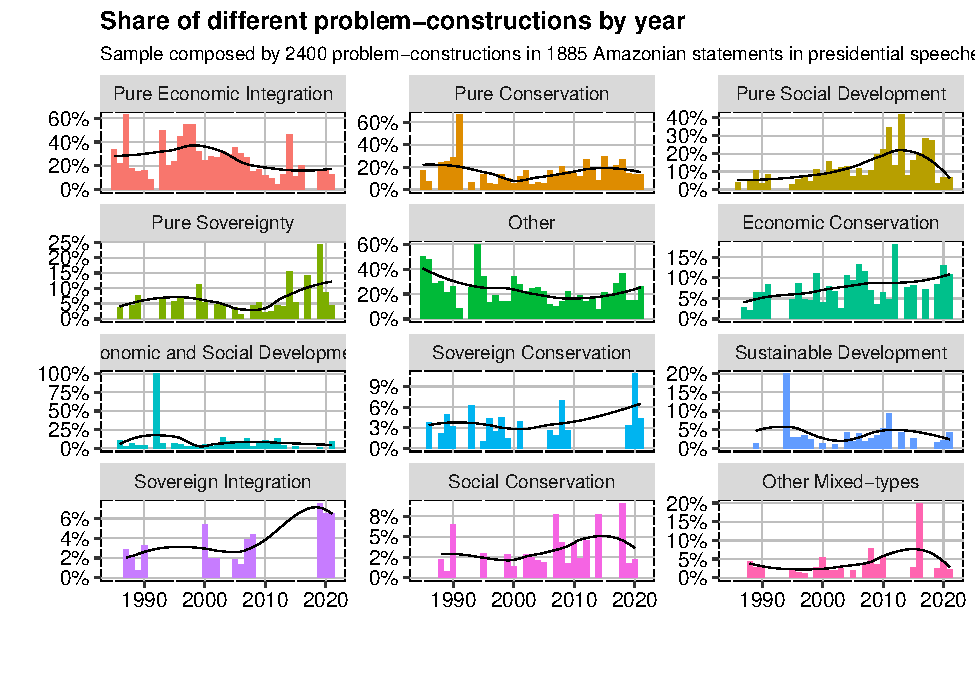
\includegraphics{Full_draft_20220401_files/figure-latex/Figure 2: mixed-types in time-1.pdf}

The plots reveal several trends. We start by pure-types. Pure economic
integration statements, which were dominant, decreased in incidence as
of the late 1990s. Concurently, pure conservation as well as pure social
development increased; both surpassing the proportion of economic
integration problem-construction in 2010. Capobianco (2021) argues that
the unprecedented decrease in deforestation we observed from 2004 to
2012 was a product of an increase in the perception of stronger federal
policies and presence in the Amazon region, which in turn engendered a
perception of higher risk of being caught and fined for deforestation.
This correlates with our findings: a higher incidence of the Amazon as a
topic overall can generate a perception of more attention from the top,
and a shift from economic integration to conservation can generate a
perception of higher change of being caught for illegal deforestation.
As of the mid 2010s, we observe a reversal of the trend with a twist:
economic integration starts picking up again in detriment of
conservation and social development problem constructions, but with
sovereignty increasing steadily.

Figure 3 (below) shows these shift and reversal more clearly and
highlights the decrease of economic integration and increase of social
and conservation problem constructions preceding Lula's presidential
mandate. Relatedly, figure 3 also shows that while the reversal precedes
the mandate of President Bolsonaro, it was with him and his dismantling
of social and environmental policies that sovereignty and economic
integration appears the most, in detriment of social development and
environmental conservation. The starkest decrease relates to social
development construction between Temer's and Bolsonaro's administration.

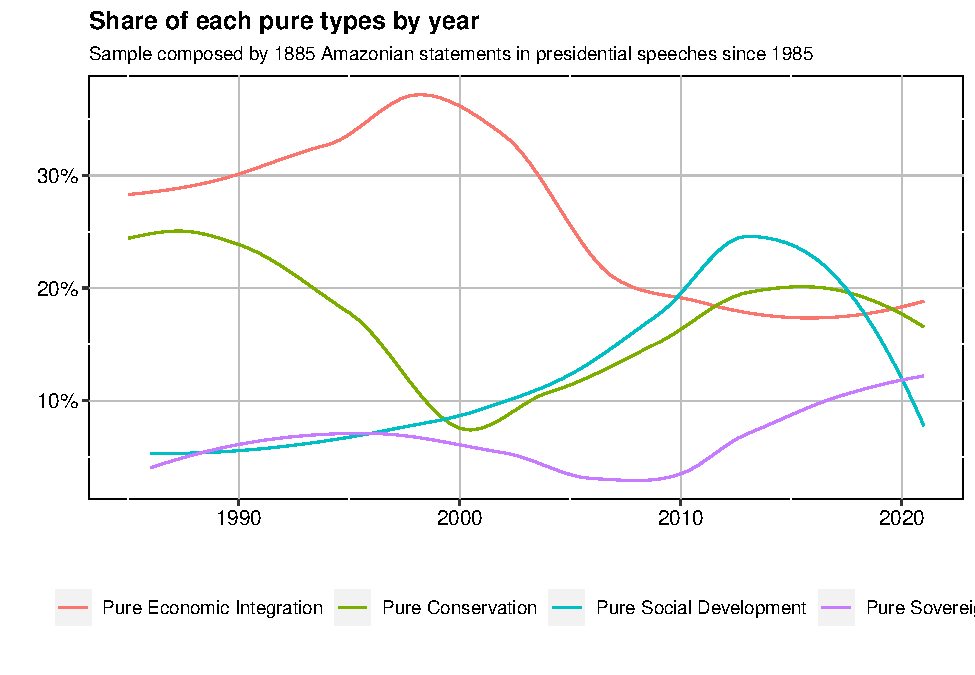
\includegraphics{Full_draft_20220401_files/figure-latex/Figure 3: pure types in time -1.pdf}

We now move to mixed types, which average at 17.7\% for all presidents
in our sample: overall, presidents prefer pure problem-constructions.
While there is some variation in time for each single mixed type, some
of them have low counts and interpretations are not adequate. We focus
our discussion on those with higher incidence. First, the most frequent
mix overall is that of economic integration with environmental
conservation, which averages at 29.15\% in relation to mixed types only,
and at 6.8\% in relation to all Amazonian statements. Overall, we
observe an increase along time, reaching its pike in the early 2010.
President Dilma was the most frequent user of this mix. A close second
is economic and social development being used together in about 22.9\%
of all mixed type statements and 5.4\% of all statements.

All other mixed types appeared less than 2.6\% on average in relation to
all statements. We can also interpret mixed types, though, by looking at
what compose them the most along time. Mixed types using conservation
were quite frequent in the lead up and aftermath of the 1992 Earth
Summit. This includes the mix type we label sustainable development,
which constructs the Amazon as a problem of economic integration, social
development, and environmental conservation. We interpret the appearance
of mixed types as more complex understandings of Amazonian problems.
This follows a global agenda of understanding interconnections of
social, environmental, and economic domains. As we show that Amazonian
incidence in discourse does respond to global issues, this is not a
surprise given agendas as Millennium Development Goals and the
Sustainable Development Goals. Nevertheless, as in pure types, we also
observe the comeback of sovereignty being used in mixed types, mostly in
detriment of conservation social development. This becomes more apparent
in a comparison between Lula and Bolsonaro, the two presidents that mix
the most with proportions 11\% above presidential averages: 29.4\% and
31.3\% respectively. While the former frequently mixed conservation with
other problem constructions, the latter prefers mixing with sovereignty.
The combination of sovereignty with economic integration, which was also
characteristic of the military dictatorship policies for the region,
reaches its highest level with Bolsonaro: 22.7\% of all mixed types.

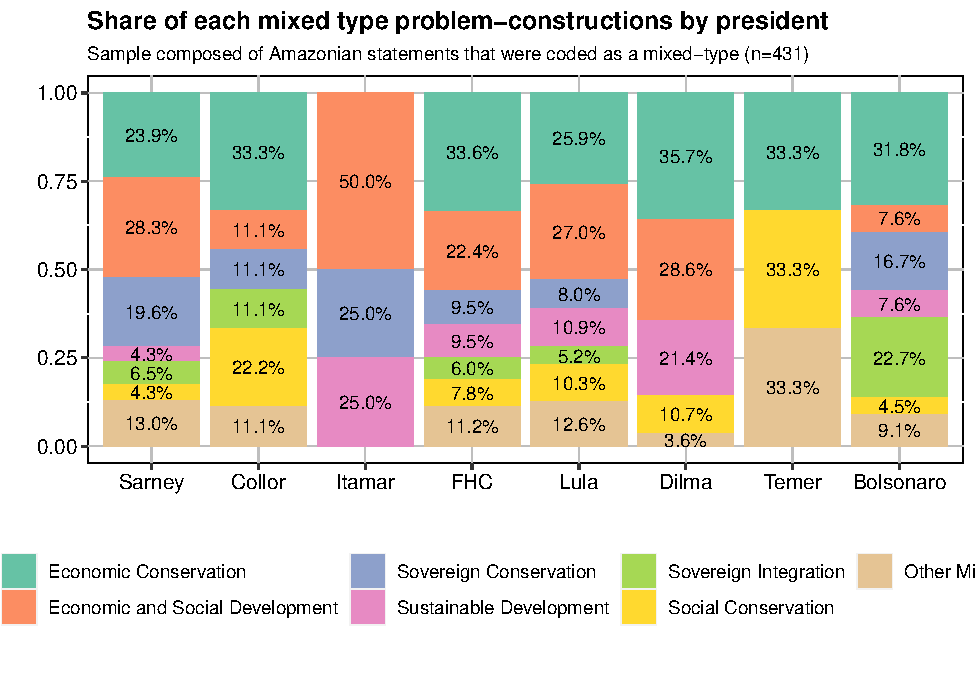
\includegraphics{Full_draft_20220401_files/figure-latex/Figure 4: mixed-types by president -1.pdf}

Pacheco (2019) proposes that we see the Amazon frontier as a key
analytic category to understand the Brazilian state and democracy.
Specifically, the author states that the natural richness of the region
has been instrumentally transformed in political support through
resource exploration by different governments over the last centuries.
The costs for said economic and political benefits are the livelihoods
of indigenous and traditional populations and the ecosystems they reside
in. Political stability, thus, can be seen as a product of the trade-off
between both. Policies during the military dictatorship were strongly
geared towards integrating the Amazon to the national territory and
international economy. With the strengthening of environmentalism in the
1990s, its most strong form being the policies adopted in the 2000s, we
can interpret the fall of economic integration and the rise of social
and conservation problem constructions as a new relationship between
granting local livelihoods their rights and economic exploitation.

While unprecedented, this new balance was not long-standing. Democratic
decay is slow and the embryo of Bolsonaro's Amazonian discourse was
breeding half a decade before he took office. We observe the decrease in
conservation related statements in the mid 2010s, and the soft increase
of sovereignty both pure and in mixes already late 2000s (figure 3) .
The hard increase in sovereignty comes in the early 2010s. As we
conceptualize and operationalize sovereignty as boundary-making
vis-à-vis internal and external perceived threats to the Amazon, we
interpret this increase as attacks to indigenous and traditional
populations. At the policy side, the Itaipu Dam in the late 2000s and
the 2011 Forest code are seen as a turning point: political opposition
to conservation got particularly organized and managed to lobby the
executive and conquer this policy wins, which were largely opposed by
environmentalists.

This is not to say that those who preceded President Bolsonaro are like
him. They are not, and we have shown how he is different from others
already. But the political forces in Brazilian democracy that drive
these changes in problem-construction were long in the making, as the
earlier and softer shifts in discourse suggest. Bolsonaro's
problem-construction is the strongest form of this shift. Now that we've
inspected and developed pure and mixed types, we can check if these
specific problem constructions vary depending on where the president is
speaking.

\hypertarget{an-amazonian-three-level-game-boasting-policy-outside-talking-to-people-inside}{%
\subsection{4.3 An Amazonian three-level game? Boasting policy outside,
talking to people
inside}\label{an-amazonian-three-level-game-boasting-policy-outside-talking-to-people-inside}}

Table 2, below, displays the multinational regression coefficients for
the correlation between diverse problem constructions and locations. The
regression coefficients express the relative probability in relation to
the reference categories, which are Amazonian states for location and
environmental conservation for problem construction. Although all the
other mixed types problem-constructions were included in the model, we
choose to display and focus the analysis on the pure types. From the
outset, we notice that problem constructions of pure economic
integration and pure social development correlate in negative
statistically significant ways to both international settings and
Brasilia in relation to environmental conservation problem constructions
in Amazonian states. These findings indicate that constructing the
Amazon as an issue of environmental conservation is more likely to
happen in international settings and in Brasilia than in Amazonian
states. Additionally, pure sovereignty correlates in negative
statistically significant ways to international settings in relation to
conservation in Amazonian states. That is, constructing the Amazon as an
issue of sovereignty is less likely in international settings than it is
in Amazonian States. Interestingly, we see no statistically significant
correlations between problem constructions in non-Amazonian states in
relation to Amazonian states. This indicates that when presidents speak
about the Amazon at the state level, constructions might be rather
similar across different states. Furthermore, we also notice that some
of the control variables correlate with some Amazonian problem
constructions in interesting ways. For example, pure sovereignty
constructions correlate negatively with election years in relation to
conservation. That is, in election years conservation constructions are
more likely to take place in comparison to sovereignty. As well, annual
deforestation rates correlate positively with economic integration
constructions in relation to conservation. This indicates that both
deforestation increases and presidents are also more likely to construct
the Amazon as an issue of economic integration.

\begin{longtable}[]{@{}llll@{}}
\caption{Table 2 - Amazon Problem-Construction by
Location}\tabularnewline
\toprule
\endhead
Dependent.Variables & Economic Integration vs.~Environmental
Conservation & Social Development vs.~Environmental Conservation &
Sovereignty vs.~Environmental Conservation \\
Brasilia.vs..Amazonian.States & -1.024*** & -1.002*** & -0.206 \\
International.vs..Amazonian.States & -0.612*** & -1.583*** &
-1.427*** \\
Non.AM.States.vs..Amazonian.States & 0.023 & -0.041 & 0.324 \\
Election.Year & -0.241 & 0.028 & -0.684** \\
Annual.Deforestation & 0.063*** & -0.031* & 0.004 \\
Average.Inflation & -0.001*** & -0.001*** & -0.0001 \\
\bottomrule
\end{longtable}

Putnam (1988) seminal article on the two level game between domestic and
international politics analyzes how negotiations at both levels make
policies possible. The author argues that both domestic and
international levels need to be taken into consideration when analyzing
how, often, domestic politics became entangled in international
negotiations. The Amazon, as a region and a forest, has been the topic
of international negotiations, national debates, and local policy
implementation; though how the Amazon has been constructed as an issue
differs on each of these three levels. While in Brasilia or
internationally different presidents might construct the Amazon as an
issue of conservation, the same presidents might construct the Amazon as
an issue of economic integration or social development at the local
level. This implies not only that audiences' priorities in each setting
change, but that which policies are appropriate to solve the ``Amazon
issue'' differ. The three level game entails that conservation might be
a desirable construction when speaking internationally about the Amazon,
but not for local electorates. Such might help explain diverse local
implementation gaps between public policy negotiated outside and
implemented within the Amazon as perceptions and expectations about the
issues the same policy addresses might differ (Alesina and Giuliano
2009; López et al. 2020).

Whereas presidential discourses at the top matter to define and justify
public policy (Zarefsky 2004), presidents shape their discourses
according to who their audience might be and what ``they want to hear''.
This democratic game contribute to the advancement of ambiguous public
policies thought from the outside to the Amazon or contradictory
policies from Amazon to the outside. Take, for example, the rural credit
offered to local agricultural producers in Amazonian states went from
500 million reais in 1999 to over 4 billion by 2012 (cite). During the
same period, the money spent in fighting deforestation in the Amazonian
states also increased from \ldots{} in \ldots{} to \ldots{} in \ldots{}
These policies match diverse local, national, and international
expectations and match solutions to different problem constructions
presented at each of these levels.

\hypertarget{conclusion}{%
\section{5 Conclusion}\label{conclusion}}

\hypertarget{references}{%
\section*{6 References}\label{references}}
\addcontentsline{toc}{section}{6 References}

\hypertarget{refs}{}
\begin{CSLReferences}{1}{0}
\leavevmode\vadjust pre{\hypertarget{ref-acker2014}{}}%
Acker, Antoine. 2014. {``{"}O maior incêndio do planeta{"}: como a
Volkswagen e o regime militar brasileiro acidentalmente ajudaram a
transformar a Amazônia em uma arena política global.''} \emph{Revista
Brasileira de História} 34 (December): 13--33.
\url{https://doi.org/10.1590/S0102-01882014000200002}.

\leavevmode\vadjust pre{\hypertarget{ref-acker2021}{}}%
---------. 2021. {``Amazon Development,''} Oxford research encyclopedia
of latin american history.,.
\url{https://doi.org/10.1093/acrefore/9780199366439.013.837}.

\leavevmode\vadjust pre{\hypertarget{ref-alesina2009}{}}%
Alesina, Alberto F., and Paola Giuliano. 2009. {``Preferences for
Redistribution.''} \url{https://www.nber.org/papers/w14825}.

\leavevmode\vadjust pre{\hypertarget{ref-andonova2014}{}}%
Andonova, Liliana B. 2014. {``Boomerangs to Partnerships? Explaining
State Participation in Transnational Partnerships for Sustainability.''}
\emph{Comparative Political Studies} 47 (3): 481--515.
\url{https://doi.org/10.1177/0010414013509579}.

\leavevmode\vadjust pre{\hypertarget{ref-assuncao2015}{}}%
Assunção, Juliano, Clarissa Gandour, and Rudi Rocha. 2015.
{``Deforestation Slowdown in the Brazilian Amazon: Prices or
Policies?''} \emph{Environment and Development Economics} 20 (6):
697--722. \url{https://doi.org/10.1017/S1355770X15000078}.

\leavevmode\vadjust pre{\hypertarget{ref-bacchi2009}{}}%
Bacchi, Carol Lee. 2009. \emph{Analysing Policy: What's the Problem
Represented to Be?} Pearson.

\leavevmode\vadjust pre{\hypertarget{ref-barros2020}{}}%
Barros, Antonio Teixeira de. 2020. {``Discursos parlamentares sobre a
Amazônia: sobre o que falam os deputados brasileiros.''} \emph{Política
\& Sociedade} 19 (46): 299--331.
\url{https://doi.org/10.5007/2175-7984.2020.e66962}.

\leavevmode\vadjust pre{\hypertarget{ref-becker2005}{}}%
Becker, Bertha K. 2005. {``Geopolítica da Amazônia.''} \emph{Estudos
Avançados} 19 (April): 71--86.
\url{https://doi.org/10.1590/S0103-40142005000100005}.

\leavevmode\vadjust pre{\hypertarget{ref-bevitori2015}{}}%
Bevitori, Cinzia. 2015. {``Discursive Constructions of the Environment
in American Presidential Speeches 1960{\textendash}2013: A Diachronic
Corpus-Assisted Study.''} \emph{Corpora and Discourse Studies}, 110--33.
\url{https://doi.org/10.1057/9781137431738_6}.

\leavevmode\vadjust pre{\hypertarget{ref-brice2021}{}}%
Brice, and Smith. 2021. {``The Amazon Is Fast Approaching a Point of No
Return.''} \emph{Bloomberg.com}, July.
\url{https://www.bloomberg.com/news/features/2021-07-29/amazon-rainforest-deforestation-land-grabs-surge-under-bolsonaro-in-brazil}.

\leavevmode\vadjust pre{\hypertarget{ref-brown2017}{}}%
Brown, George, and Benjamin K. Sovacool. 2017. {``The Presidential
Politics of Climate Discourse: Energy Frames, Policy, and Political
Tactics from the 2016 Primaries in the United States.''} \emph{Energy
Policy} 111 (December): 127--36.
\url{https://doi.org/10.1016/j.enpol.2017.09.019}.

\leavevmode\vadjust pre{\hypertarget{ref-calderwood2019}{}}%
Calderwood, Kevin J. 2019. {``Discourse in the Balance: American
Presidential Discourse about Climate Change.''} \emph{Communication
Studies} 70 (2): 235--52.
\url{https://doi.org/10.1080/10510974.2019.1572636}.

\leavevmode\vadjust pre{\hypertarget{ref-calderwood2020}{}}%
---------. 2020. {``Going Global: Climate Change Discourse in
Presidential Communications.''} \emph{Environmental Communication} 14
(1): 52--67. \url{https://doi.org/10.1080/17524032.2019.1592005}.

\leavevmode\vadjust pre{\hypertarget{ref-campbell2015}{}}%
Campbell, Jeremy M. 2015. \emph{Conjuring Property: Speculation and
Environmental Futures in the Brazilian Amazon}. Illustrated edition.
Seattle: University of Washington Press.

\leavevmode\vadjust pre{\hypertarget{ref-capobianco2019}{}}%
Capobianco, João Paulo. 2019. {``Avances y retrocesos de la
sostenibilidad en la Amazonia: un análisis de la gobernanza
socioambiental en la Amazonia,''} January.
\url{https://gredos.usal.es/handle/10366/139311}.

\leavevmode\vadjust pre{\hypertarget{ref-capobianco2021}{}}%
---------. 2021. \emph{Amazônia: Uma Década de Esperança}. 1ª edição.
São Paulo: Estação Liberdade.

\leavevmode\vadjust pre{\hypertarget{ref-cezar2020}{}}%
Cezar, Rodrigo Fagundes. 2020. {``Brazilian Presidential Speeches from
1985 to July 2020.''}
\url{https://dataverse.harvard.edu/dataset.xhtml?persistentId=doi:10.7910/DVN/M9UU09}.

\leavevmode\vadjust pre{\hypertarget{ref-drummond2006}{}}%
Drummond, Jose, and Ana Flavia Barros-Platiau. 2006. {``Brazilian
Environmental Laws and Policies, 1934-2002: A Critical Overview.''}
\emph{Law \textless Html{\_}ent Glyph={"}@amp;{"}
Ascii={"}\&amp;{"}/\textgreater{} Policy} 28 (1): 83--108.
\url{https://doi.org/10.1111/j.1467-9930.2005.00218.x}.

\leavevmode\vadjust pre{\hypertarget{ref-fearnside1990}{}}%
Fearnside, Philip M. 1990. {``The Rate and Extent of Deforestation in
Brazilian Amazonia.''} \emph{Environmental Conservation} 17 (3):
213--26. \url{https://doi.org/10.1017/s0376892900032355}.

\leavevmode\vadjust pre{\hypertarget{ref-franchini2019}{}}%
Franchini, Matias Alejandro, and Eduardo Viola. 2019. {``Myths and
Images in Global Climate Governance, Conceptualization and the Case of
Brazil (1989 - 2019).''} \emph{Revista Brasileira de Política
Internacional} 62 (September).
\url{https://doi.org/10.1590/0034-7329201900205}.

\leavevmode\vadjust pre{\hypertarget{ref-garfield2013}{}}%
Garfield, Seth. 2013. \emph{In Search of the Amazon: Brazil, the United
States, and the Nature of a Region}. Durham: Duke University Press
Books.

\leavevmode\vadjust pre{\hypertarget{ref-harris2021}{}}%
Harris, Bryan. 2021. {``Drought Puts Amazon at Risk of {`}Large-Scale
Dieback{'}, Researchers Warn.''} \emph{Financial Times}, July.
\url{https://www.ft.com/content/02071ae7-dcf5-4c61-9c3c-b55f5aef8b0e}.

\leavevmode\vadjust pre{\hypertarget{ref-hecht2013}{}}%
Hecht, Susanna B. 2013. \emph{The Scramble for the Amazon and the
{"}Lost Paradise{"} of Euclides Da Cunha}. First edition. Chicago:
University of Chicago Press.

\leavevmode\vadjust pre{\hypertarget{ref-hecht1990}{}}%
Hecht, Susanna B., and Alexander Cockburn. 1990. \emph{The Fate of the
Forest: Developers, Destroyers, and Defenders of the Amazon, Updated
Edition}. Chicago, IL: University of Chicago Press.
\url{https://press.uchicago.edu/ucp/books/book/chicago/F/bo10387801.html}.

\leavevmode\vadjust pre{\hypertarget{ref-hirschman1963}{}}%
Hirschman, Albert O. 1963. \emph{Journeys Toward Progress: Studies of
Economic Policy-Making in Latin America}. Twentieth Century Fund.

\leavevmode\vadjust pre{\hypertarget{ref-hirschman1975}{}}%
---------. 1975. {``Policymaking and Policy Analysis in Latin America: A
Return Journey.''} \emph{Policy Sciences} 6 (4): 385--402.
\url{https://www.jstor.org/stable/4531616}.

\leavevmode\vadjust pre{\hypertarget{ref-hochstetler2021}{}}%
Hochstetler, Kathryn. 2021. {``Climate Institutions in Brazil: Three
Decades of Building and Dismantling Climate Capacity.''}
\emph{Environmental Politics} 30 (sup1): 49--70.
\url{https://doi.org/10.1080/09644016.2021.1957614}.

\leavevmode\vadjust pre{\hypertarget{ref-hochstetler2007}{}}%
Hochstetler, Kathryn, and Margaret E. Keck. 2007. \emph{Greening Brazil:
Environmental Activism in State and Society}.
\url{https://doi.org/10.1215/9780822390596}.

\leavevmode\vadjust pre{\hypertarget{ref-lopez2020}{}}%
López, Matias, Graziella Moraes Silva, Chana Teeger, and Pedro Marques.
2020. {``Economic and Cultural Determinants of Elite Attitudes Toward
Redistribution.''} \emph{Socio-Economic Review}, May.
\url{https://doi.org/10.1093/ser/mwaa015}.

\leavevmode\vadjust pre{\hypertarget{ref-meyer2021}{}}%
Meyer, David, Evgenia Dimitriadou, Kurt Hornik, Andreas Weingessel, and
Friedrich Leisch. 2021. \emph{E1071: Misc Functions of the Department of
Statistics, Probability Theory Group (Formerly: E1071), TU Wien}.
\url{https://CRAN.R-project.org/package=e1071}.

\leavevmode\vadjust pre{\hypertarget{ref-miranda2021}{}}%
Miranda, David. 2021. {``Bolsonaro{'}s 1,000km Amazon Railway Will Cause
Climate Chaos. It Must Be Stopped.''} \emph{The Guardian}, July.
\url{https://www.theguardian.com/commentisfree/2021/jul/28/bolsonaro-amazon-railway-climate-chaos-must-be-stopped}.

\leavevmode\vadjust pre{\hypertarget{ref-noble2006}{}}%
Noble, William S. 2006. {``What Is a Support Vector Machine?''}
\emph{Nature Biotechnology} 24 (12): 1565--67.

\leavevmode\vadjust pre{\hypertarget{ref-pacheco2019}{}}%
Pacheco, João. 2019. \emph{Ecxterminio y Tutela: Procesos de Formación
de Alteridades En El Brasil}. UNSAM Edita. Ciencias sociales.
\url{http://www.unsamedita.unsam.edu.ar/product/exterminio-y-tutela-procesos-de-formacion-de-alteridades-en-el-brasil/}.

\leavevmode\vadjust pre{\hypertarget{ref-putnam1988}{}}%
Putnam, Robert D. 1988. {``Diplomacy and Domestic Politics: The Logic of
Two-Level Games.''} \emph{International Organization} 42 (3): 427--60.
\url{http://www.jstor.org/stable/2706785}.

\leavevmode\vadjust pre{\hypertarget{ref-silva-muller2022}{}}%
Silva-Muller, Livio, and Moira Faul. 2022. {``Protecting the Amazon and
Its People: The Role of Civil Society in the Local Effectiveness of
Transnational Partnerships.''} In, 1st ed., 288. Routledge Research in
Environmental Policy and Politics. Taylor; Francis Routledge.
\url{https://www.routledge.com/Partnerships-for-Sustainability-in-Contemporary-Global-Governance-Pathways/Andonova-Faul-Piselli/p/book/9780367708870\#:~:text=\%22Partnerships\%20for\%20Sustainability\%20provides\%20a,collaboration\%20of\%20public\%20and\%20private.}

\leavevmode\vadjust pre{\hypertarget{ref-simons1988}{}}%
Simons, Marlise, and Special To the New York Times. 1988. {``Vast Amazon
Fires, Man-Made, Linked to Global Warming.''} \emph{The New York Times},
August.
\url{https://www.nytimes.com/1988/08/12/world/vast-amazon-fires-man-made-linked-to-global-warming.html}.

\leavevmode\vadjust pre{\hypertarget{ref-lepolaindewaroux2021}{}}%
Waroux, Yann de, Rachael D. Garrett, Mollie Chapman, Cecilie Friis,
Jeffrey Hoelle, Leonie Hodel, Kelly Hopping, and Julie Gwendolin
Zaehringer. 2021. {``The Role of Culture in Land System Science.''}
\emph{Journal of Land Use Science} 16 (4): 450--66.
\url{https://doi.org/10.1080/1747423X.2021.1950229}.

\leavevmode\vadjust pre{\hypertarget{ref-westerwinter2021}{}}%
Westerwinter, Oliver. 2021. {``Transnational Public-Private Governance
Initiatives in World Politics: Introducing a New Dataset.''} \emph{The
Review of International Organizations} 16 (1): 137--74.
\url{https://doi.org/10.1007/s11558-019-09366-w}.

\leavevmode\vadjust pre{\hypertarget{ref-zarefsky2004}{}}%
Zarefsky, David. 2004. {``Presidential Rhetoric and the Power of
Definition.''} \emph{Presidential Studies Quarterly} 34 (3): 607--19.
\url{https://www.jstor.org/stable/27552615}.

\end{CSLReferences}

\end{document}
